\documentclass[linedtoc,
               parskip,
               twoside,
               longdoc,
               11pt,
               noheadingspace,
               accentcolor=tud1d,
               bigchapter,
               %draft,
               colorback]{tudreport}

%% language
\usepackage[english]{babel}
\usepackage[utf8]{inputenc}
%\usepackage[ansinew]{inputenc}  % Input-Encodung: ansinew for Windows
\usepackage{microtype} % optischer Randausgleich bei pdflatex mit Zeichendehnung

%% table
\usepackage{booktabs}
\usepackage{multirow}
\usepackage{longtable}
\usepackage{tabularx}

%% State Chart
\usepackage{pgf}
\usepackage{tikz}

%% matematics
\usepackage{amsmath}
\usepackage{nicefrac}
\usepackage{icomma}

%% misc
\usepackage{paralist}% erweiterte Listenumgebung (z.B. compactitem)
\usepackage{textcomp} % verschiedene Symbole
\usepackage[nottoc, numbib]{tocbibind}
\usepackage[ngerman]{hyperref}
\renewcommand\plparsep{1ex}
\usepackage{enumerate}
\usepackage[stable]{footmisc}

\hypersetup{%
  pdftitle={Seminar},
  pdfauthor={Harini Venkataramani},
  pdfsubject={IMPLEMENTATION AND ANALYSIS OF A FIELD
PROGRAMMABLE ADC DESIGN FOR THE INTERFACING OF
FPGAS},
  pdfview=FitH,
  pdfstartview=FitV
}

%%% Zum Tester der Marginalien %%%
  \newif\ifTUDmargin\TUDmarginfalse
  %%% Wird der Folgende Zeile einkommentiert,
  %%% werden Marginalien gesetzt.
  % \TUDmargintrue
  \ifTUDmargin\makeatletter
    \TUD@setmarginpar{2}
  \makeatother\fi
%%% ENDE: Zum Tester der Marginalien %%%

\newlength{\longtablewidth}
\setlength{\longtablewidth}{0.7\linewidth}
\addtolength{\longtablewidth}{-\marginparsep}
\addtolength{\longtablewidth}{-\marginparwidth}


% \settitlepicture{tudreport-pic}
% \printpicturesize

\title{IMPLEMENTATION AND ANALYSIS OF A FIELD
PROGRAMMABLE ADC DESIGN FOR THE INTERFACING OF
FPGAS}
\subtitle{Master Thesis: Harini Venkataramani}
\subsubtitle{Supervisor: Dipl.-Ing. Oliver Bachmann\\
  Start Date: 2nd May 2018 \textbar\ Submission Date: 1st Nov. 2018\\
  Fachgebiet Integrierte Elektronische Systeme\hfill\textbar\hfill Prof.\,Dr.-Ing.\, Klaus Hofmann}
\setinstitutionlogo{logo/ies_logo}
%\institution{Institut f"ur Datentechnik \\ Fachgebiet Rechnersysteme \\ Prof.\,Dr.-Ing.\, Hans Eveking}
%\settitlepicture{images/spartan}
\begin{document}

%% Titel %%%%%%%%%%%%%%%%%%%%%%%%%%%%%%%%%%%%%%%%%%%%%%%%%%%%%%%%%%%%%%%%%%
\maketitle
\cleardoublepage

%% Vorgeplnkel %%%%%%%%%%%%%%%%%%%%%%%%%%%%%%%%%%%%%%%%%%%%%%%%%%%%%%%%%%%%%%
\pagestyle{empty}
\pagenumbering{roman}

%% Inhaltsverzeichnis%%%%%%%%%%%%%%%%%%%%%%%%%%%%%%%%%%%%%%%%%%%%%%%%%%%%%%%%%%%
\pagestyle{plain}
\tableofcontents
\cleardoublepage


%% Hauptteil %%%%%%%%%%%%%%%%%%%%%%%%%%%%%%%%%%%%%%%%%%%%%%%%%%%%%%%%%%%%%%%
\pagestyle{headings}
\pagenumbering{arabic}
%
%\chapter{Einleitung}
\label{cha:einleitung}

TEX/LATEX ist ein "au"serst flexibles, rechner- und betriebssystemunabh"angiges Satzsystem, das zur 
Erstellung von Dokumenten in Buchdruckqualit"at geeignet ist. Von der Anfertigung kompletter 
B"ucher "uber wissenschaftliche Publikationen, mathematische Formeln, Zeitungsartikel, bis hin 
zu Briefen, Folien und vieles mehr k"onnen Sie Ihre Texte entweder dem Standardlayout von 
TEX/LATEX anvertrauen oder selbst Ihre individuellen Gestaltungsw"unsche einbringen.  

\section{Formatierung der Vorlage}
\label{sec:formatierung}


Die in dieser Vorlage festgelegte Formatierung ist an der Formatierung des Instituts f"ur Datentechnik angepasst 
und hat als Ziel den Studenten die Erstellung der Diplom-, Studien-, Master- oder Bacherlorarbeit zu erleichtern.
Mit Hilfe der vorliegenden Anleitung werden dem Nutzer das Erstellen von Texte, Formeln und Fu"snoten sowie das Einf"ugen von Randbemerkungen, Tabellen, Graphiken, Verzeichnisse und einiges mehr erl"autert. 



%\chapter{"Uberschriften}
\label{cha:uberschriften}

F"ur solch eine Arbeit wird der Text in diverse Abschnitte, Unterabschnitte und evtl. auch noch Unterunterabschnitte unterteilt. Diese m"ussen dann mit der entsprechenden "Uberschrift gekennzeichnet werden. Die Dokumentklasse parkskip kennt hier die Unterscheidung in chapter, section, subsection, subsubsection und paragraph.

Der Befehl {\textbackslash chapter\{"Uberschrift1\}} beginnt ein neues Kapitel, erzeugt eine Kapitel"uberschrift und tr"agt diese ins Inhaltsverzeichnis ein. So ist der oben genante Kapitel mit dem Befehl {\textbackslash chapter\{"Uberschriften\}} als chapter definiert.

Optional kann man mit Hilfe des Befehls {\textbackslash chapter[Kurzform]\{"Uberschrift\}} eine Kurzform f"ur den Kapitelname angeben. Die Kurzform wird dann anstelle der "Uberschrift ins Inhaltsverzeichnis eingetragen.
\paragraph{Beispiel}
\label{par:beispiel}

{\textbackslash chapter[Anf"ange (1920)]\{Anf"ange der modernen Science--Fiction--Literatur (1920)\}}. Im Inhaltsverzeichnis erscheint nur "Anf"ange (1920)".

\section{"Uberschrift2}
\label{sec:uberschrift2}

Mit dem Befehl {\textbackslash section\{"Uberschrift2\}} wird einen neuen Abschnitt des Dokuments auf der section-Ebene erzeugt. Die zugeh"orige "Uberschrift wird definiert und ins Inhaltsverzeichnis eingetragen. Wenn eine Kurzform erw"unscht ist, kann sie auch mit dem entsprechenden Befehl erzeugt werden (Siehe Beispiel unter Kapitel\ref{par:beispiel}).

\subsection{"Uberschrift3}
\label{sec:uberschrift3}

In der subsection-Ebene, wird ebenfalls die zugeh"orige "Uberschrift erzeugt und ins Inhaltsverzeichnis eingetragen. Hier ist auch ebenfalls m"oglich eine Kurzform angegeben. Der Befehl lautet folgenderma"sen {\textbackslash subsection\{"Uberschrift3\}}.

\subsubsection{"Uberschrift4 und Paragraph}
\label{sec:uberschrift4}

Der Befehle dazu lauten {\textbackslash subsubsection\{"Uberschrift4\}} bzw. {\textbackslash paragraph\{"Paragraph\}}. Die "Uberschriften f"ur diese Ebenen erfolgen ohne Nummerierung und werden nicht im Inhaltsverzeichnis aufgenommen. Das o.g. Beispiel wurde z. B. als Paragraph definiert.






%\chapter{Text in Latex}
\label{cha:text}

In Latex gibt es f"ur einige Symbole bestimmte Befehle die man eingeben muss um sie als Text richtig darstellen zu k"onnen. Im folgenden werden einige Befehle bzw. Codierungen zur Erstellung einiger Symbole erl"autert. 


%% Umlaute Seite %%%%%%%%%%%%%%%%%%%%%%%%%%%%%%%%%%%%%%%%%%%%%%%%%%%%%%%%%%%%%%%%
\section{Umlaute und "Ahnliches}
\label{sec:umlaute}

Es gibt einige Methoden Umlaute in Latex zu setzten. Die einfachste erfolgt mit Hilfe eines Anf"urungszeichens, das vor dem gew"unschten Vokal positioniert werden muss, d.h. um das Wort ``K"uhe'' richtig darzustellen muss man im Editor ``K''uhe'' schreiben. Genauso werden auch die Umlaute "a und "o erzeugt.\\F"ur scharfes s `` "s '' braucht man auch vor einem ``s'' wieder ein Anf"uhrungszeichen zu setzten.
\\
Die Codierung bzw. entsprechenden Befehle zu weiteren Sonderzeichen kann man unter \href{[http://de.wikibooks.org/wiki/LaTeX-Kompendium:_Sonderzeichen]}{www.wikibooks.org} finden.\\
\\

\section{Querverweis}
\label{sec:ref}
Innerhalb eines Textes kann man einen Querverweis einf"ugen. Dies funktioniert mit dem Befehl {\textbackslash ref \{Name\}}. Der Befehl erzeugt einen Querverweis auf eine Textstelle, die zuvor durch einen {\textbackslash label}-Befehl mit dem angegebenen Namen versehen wurde. Der Querverweis gibt die Gliederungsnummer der betreffenden Textstelle an. Aus diesem Grund es ist sinnvoll Kapiteln bzw. Unterkapiteln auf die man "ofter verweisen m"ochte mit dem Befehl {\textbackslash label\{Name\} zu vermerken. 
 
 \paragraph{Beispiel}
 
 Siehe Kapitel \ref{cha:text} um ausf"uhrliche Information zum Text in Latex.
 
 In diesem Beispiel wurde auf den Kapitel Text in Latex verwiesen mit {\textbackslash ref\{text\}} da das Kapitel Text in Latex mit dem Befehl {\textbackslash label\{cha:text\}} versehen wurde. Der Befehl {\textbackslash label} muss direkt nach dem Befehl f"ur den Gliederungsabschnitt bzw. "Uberschrift erfolgen.
 
 
%\chapter{Formeln in Latex}
\label{cha:formeln}


Im prinzip ist die Syntax relativ einfach aufgebaut. Wenn man eine Formel in LaTeX eingeben m"ochte, muss eine entsprechende Umgebung gew"ahlt werden. Es gibt mehrere, die bekanntesten sind math und displaymath. 
\begin{itemize}
\item displaymath setzt die Formel ab und zentriert sie 
\item math baut die Formel mehr in den Text ein.
\end{itemize}

Eingeleitet wird eine solche Umgebung durch {\textbackslash begin} also z.B. {\textbackslash begin\{displaymath\}} und durch {\textbackslash end} beendet. Anhand folgenden Beispiels  l"asst sich zeigen wie ein Bruch aufbaut und dargestellt wird. \\
\\
Mit den Befehlen,\\
\\
\textbackslash begin\{math\}\\
\textbackslash frac\{1\}\{2\}  \\
\textbackslash end\{math\}\\
\\
wird der Bruch 
\begin{math} 
\frac{1}{2} 
\end{math} 
mitten im Text erscheinen. Gibt man die Befehle,\\
\\
\textbackslash begin\{displaymath\}\\
\textbackslash frac\{1\}\{2\}  \\
\textbackslash end\{displaymath\}\\
\\
erscheint der Bruch zentriert als separate Formel, n"amlich,
\begin{displaymath} 
\frac{1}{2} 
\end{displaymath} 

Andere Konstruktionselemente lassen sich besser an konkreten Formeln darstellen. Daher hier einige bekannte Formel aus Naturwissenschaft und Statistik.
	
\vspace{1cm} 
Formel f"ur das arithmetische Mittel einer Stichprobe: 
\begin{displaymath} 
\bar{x} = \frac{1}{n} \sum_{i=1}^{n} x_i 
\end{displaymath} 
Formel f"ur die Varianz einer Stichprobe: 
\begin{displaymath} 
s^2 = \frac{1}{n-1} \sum_{i=1}^{n} (x_i - \bar{x}) 
\end{displaymath} 
Formel f"ur die Standardabweichung: 
\begin{displaymath} 
s = \sqrt{s^2} = \sqrt{\frac{1}{n-1} \sum_{i=1}^{n} (x_i - \bar{x})^2} 
\end{displaymath} 
oder: 
\begin{displaymath} 
= \sqrt{\frac{ \sum_{i=1}^{n} (x_i - \bar{x})^2}{n-1}} 
\end{displaymath} 
Geometrisches Mittel: 
\begin{displaymath} 
G = \sqrt[n]{ \prod^n_{i=1} x_i} 
\end{displaymath} 
Binomialkoeffizient: 
\begin{displaymath} 
{n \choose k} = \frac{ n! }{ k! (n-k) !} 
\end{displaymath} 
Zeitunabh"angige dreidimensionale Schr"odingergleichung: 
\begin{displaymath} 
\frac{\partial^2 \psi}{\partial x ^2} + \frac{\partial^2 \psi}{\partial y ^2} + \frac{\partial^2 \psi}{\partial z ^2} = - \frac{2m}{\hbar^2}(E -U)\psi. 
\end{displaymath} 
Faradaysches Induktionsgesetz: 
\begin{displaymath} 
\oint \bf{E} \cdot ds = -\int \frac{\partial \mathcal{B}}{\partial t} \cdot \bf{A} 
\end{displaymath} 


%\chapter{Einbindung von Graphen}
\label{cha:graph}

Um Bilder in Latex einzubinden es ist nur wichtig dass sie im richtigen Format und im richtigen Verzeichnis vorliegen. Unter dem Ordner `` Dokumentation'' f"ur diese Vorlage ist der Unterordner `` images '' angelegt. In diesem Ordner liegen alle Bilder die in diesem Dokument enthalten sind. Da k"onnen auch alle Bilder angelegt werden die in der Arbeit aufgerufen werden sollen. Die Bilder sollen f"ur diese Vorlage in .pdf oder .jpg vorliegen. Die Bilder k"onnen auch direkt im Hauptverzeichnis angelegt werden.
\\Anhand folgenden Beispiels werden die Befehle erl"autert die man braucht um ein Bild in diesem Kapitel hinzuzuf"ugen. 

\paragraph{Beispiel}

Das Bild mit dem Namen `` blockschaltbild.pdf '', das im Unterordner `` images '' liegt, wird mit folgenden Befehlen aufgerufen,

 {\textbackslash begin\{figure\}[ht]}
\\	{\textbackslash centering}
\\		{\textbackslash includegraphics[width=0.66\textbackslash textwidth]\{images/blockschaltbild.pdf\}}
\\	{\textbackslash caption\{Beispiel: Blockschaltbild \cite{guo}}}
\\	{\textbackslash label\{fig:blockschaltbild\}}
\\ {\textbackslash end\{figure\}}


\begin{figure}[!ht]
	\centering
		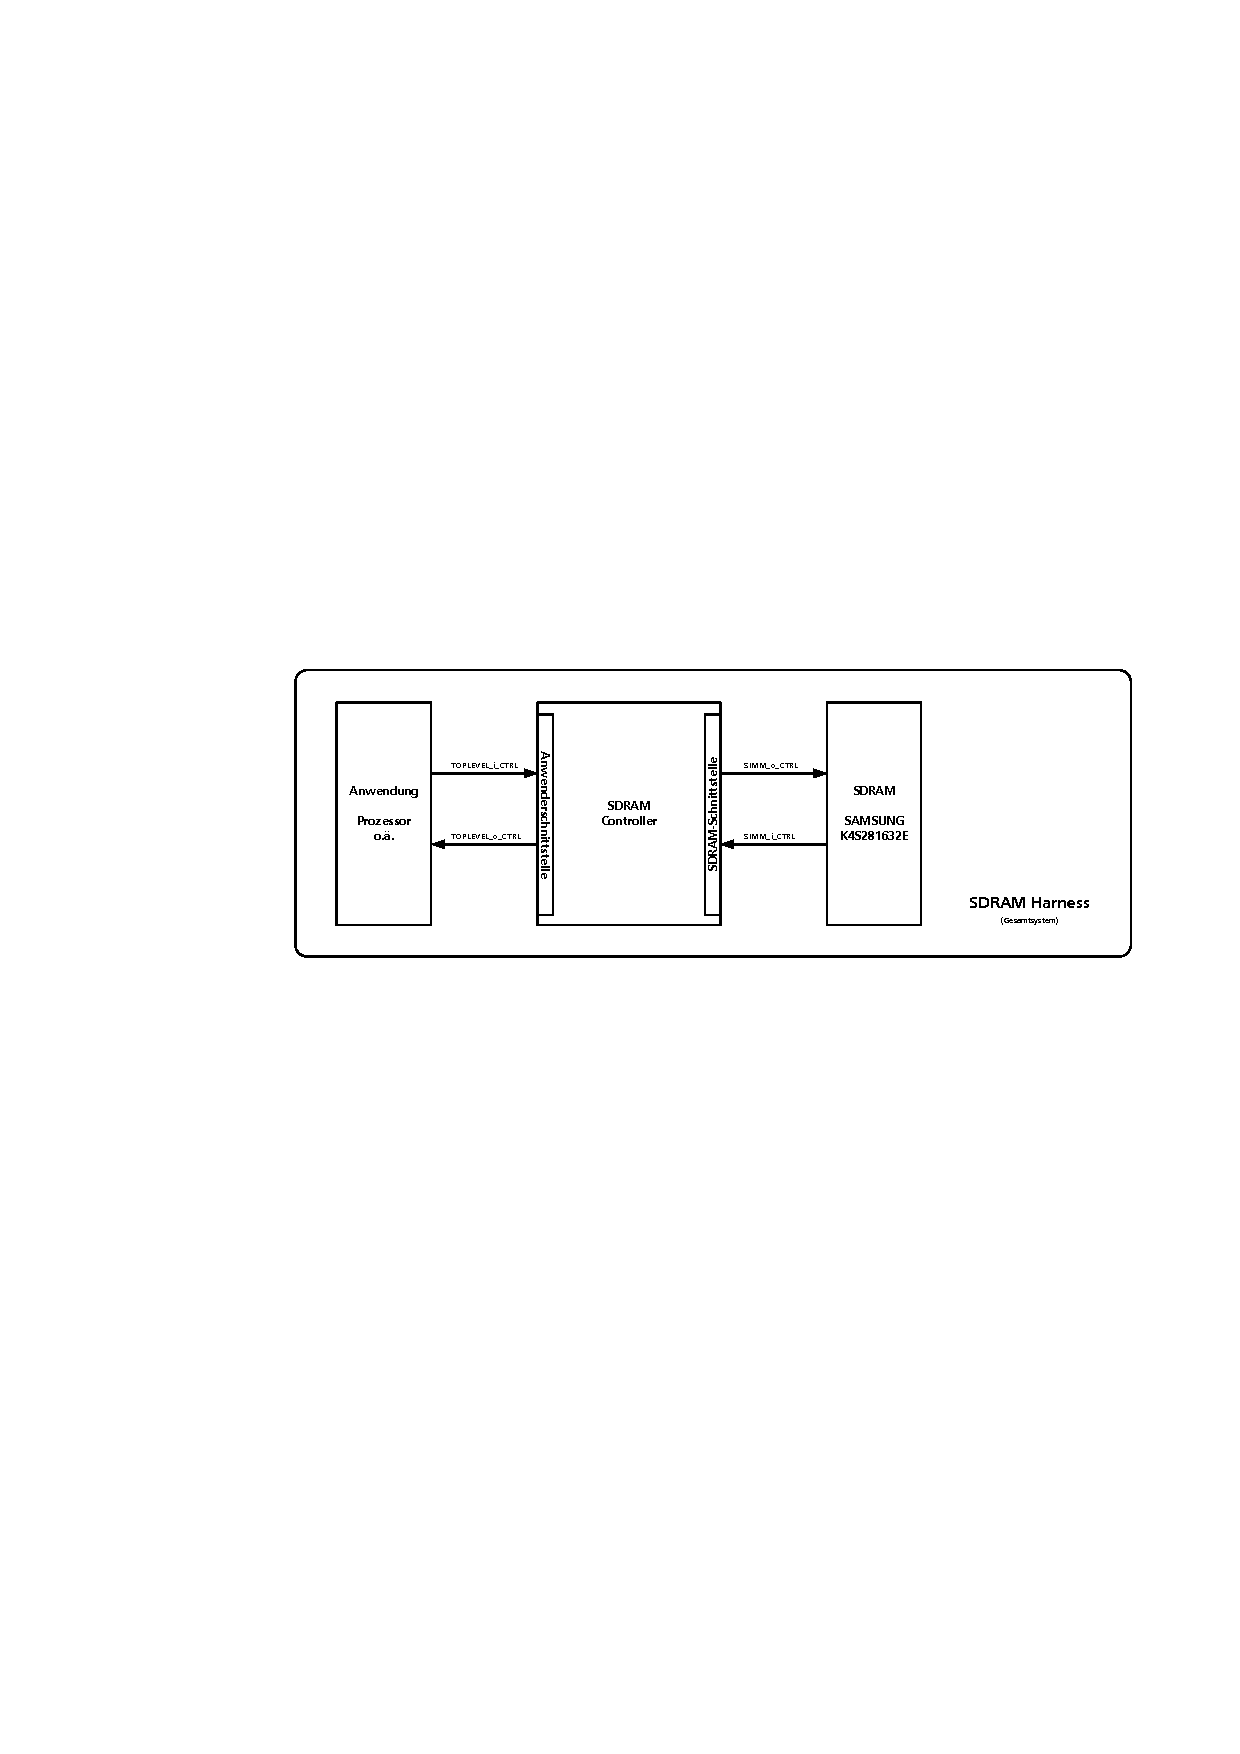
\includegraphics[width=0.66\textwidth]{images/blockschaltbild.pdf}
	\caption{Beispiel: Blockschaltbild \cite{guo}}
	\label{fig:blockschaltbild}
\end{figure}

%\begin{figure}[ht]
%	\centering
%		\includegraphics[width=1.00\textwidth]{images/busy-konflikt.jpg}
%	\caption{Busy-Konflikt im Einzelzugriff.}
%	\label{fig:busy-konflikt}
%\end{figure}

%\chapter{Tabellen}
\label{cha:tabellen}

Um eine einfache Tabelle in Latex zu erzeugen, kann man sich zun"achst mit der tabular-Umgebung begn"ugen. Die Syntax daf"ur ist die folgende: \\
 \\
\textbackslash begin \{tabular\}\{cols\} \\
Tabelleneintr"age \\
\textbackslash end\{tabular\}\\
 \\
Im Argument ``cols'' gibt man f"ur jede Spalte, die in der Tabelle stehen soll, die Ausrichtung 
an. Man hat dabei folgende Optionen: 
 
\begin{table}[htp]
\centering
\begin{tabular}{|c|c|}
\hline
l&Linksb"undig\\
\hline
r&Rechtsb"undig\\
\hline
c&Zentriert\\
\hline
p\{x cm\}&Parbox der Breite x cm\\
\hline
\end{tabular}

\caption{Tabellenausrichtung}
\label{tab:Ausrichtung}
\end{table}

 
Will man die Spalten durch einen oder mehrere Striche trennen, so f"ugt man mittels der 
Tastenkombination AltGr + ``<'' einen senkrechten Strich (|) zwischen (bzw. vor oder nach) 
den Ausrichtungsangaben ein (siehe Beispiele).  
Die Breite der Spalten bestimmt LATEX selbst, es sei denn man gibt eine Parbox an. Die 
Parbox hat den weiteren Vorteil, dass in einer Zelle der Tabelle mehrere Zeilen m"oglich sind. 
Weiters kann man mittels Parboxen auch Tabulatoren wie im Word erzeugen. 
 
Die Tabelleneintr"age werden zeilenweise eingegeben. Dabei erfolgt die Trennung innerhalb 
der Zeile mit ``\&''. Um in die n"achste Zeile zu springen hat man den Befehl ``\textbackslash \textbackslash''. Will man 
auch die Zeilen mittels Strichen trennen, so sind diese mit dem Befehl``\textbackslash hline'' an die 
entsprechende Stelle zu setzen.  
 
Das folgenden Beispiele erl"autern die tabular-Umgebung:  
Mit diesen Kommandos 

\textbackslash begin\{tabular\}\{1p\{10cm\}\}\\
\textbackslash textbf\{tabular\} \& Die Umgebung tabular wird in Latex gew"alt um einfache Tabellen zu erzeugen\textbackslash\textbackslash\\
\textbackslash textbf\{table\} \& table wird gebraucht um abgesetzte Tabellen zu erzeugen. Die Tabelle kann damit als Gleitobjekt eingef"ugt werden\textbackslash\textbackslash\\
\textbackslash textbf\{hline\} \& Mit diesem Befehl kann man mit einem Strich Zeilen trennen\textbackslash\textbackslash\\
\textbackslash textbf\{\textbackslash textbackslash\textbackslash textbackslash\} \& Um auf die n"achste Zeile zu springen\textbackslash\textbackslash\\
\textbackslash end \{tabular\}\textbackslash\textbackslash\\
\\
wird folgende Tabelle erzeugt:\\

\begin{tabular}{lp{10cm}}
\textbf{tabular} & Die Umgebung tabular wird in Latex gew"alt um einfache Tabellen zu erzeugen\\
\textbf{table}& table wird gebraucht um abgesetzte Tabellen zu erzeugen. Die Tabelle kann damit als Gleitobjekt eingef"ugt werden\\
\textbf{hline}& Mit diesem Befehl kann man mit einem Strich Zeilen trennen\\
\textbf{\textbackslash\textbackslash}& Um auf die n"achste Zeile zu springen\\
\end {tabular}\\
\\
\\
Dies ist ein Beispiel, wie man Parboxen zur ``Erzeugung'' von Tabulatoren benutzt werden 
kann. \\
\\
Tabellen, welche mittels der tabular-Umgebung geschrieben werden, werden einfach, wie ein 
gro"ser Buchstabe in den Text eingef"ugt. Um abgesetzte Tabellen zu erzeugen bedient man 
sich zus"atzlich der table-Umgebung, die die Tabelle als sogenanntes Gleitobjekt einf"ugt. Sie 
hat folgende Syntax: 
 
\textbackslash begin\{table\}[Ausrichtung] \\
tabular-Umgebung \\
\textbackslash end\{table\}\\ 
\\
In die eckigen Klammern steht die Ausrichtung. Daf"ur hat man folgende Optionen: 

\begin{table}[h]
\begin{center}
\begin{tabular}{|l|p{8cm}|}
\hline
h&``here''- Tabelle soll an der selben Stelle wie im Quelltext eingerichtet werden\\
\hline
t&``top''- Tabelle wird an den unteren Rand der Seite gestellt\\
\hline
b&``bottom''- Tabelle wird an den unteren Rand der Seite gestellt\\
\hline
p&``page''- Tabelle wird auf einer Gleitobjektseite eingerichtet\\
\hline
\end{tabular}
\end{center}
\caption{table-Ausrichtung }
\label{tab: table Ausrichtung}
\end{table}%

\paragraph{Weiteres Beispiel}
 
Die folgenden Befehle erzeugen eine Tabelle mit Linien: 

\textbackslash begin\{table\}[!h]\\
\textbackslash begin\{center\}\\
\textbackslash begin\{tabular\}\{|l|r|r|r|r|r|\}\\
\textbackslash hline\&\$x\_\{min\}\$\&\$x\_\{0,25\}\$\&\$x\_\{0,5\}\$\&\$x\_\{0,75\}\$\&\$x\_\{max\}\$\textbackslash\textbackslash\\
\textbackslash hline
\textbackslash hline Alter \&14\&19\&20,5\&23\&70\textbackslash\textbackslash\\
\textbackslash hline Semester \&0\&2\&2\&4\&14\textbackslash\textbackslash\\
\textbackslash hline
\textbackslash end\{tabular\}\\


\begin{table}[h]
\begin{center}
\begin{tabular}{|l|r|r|r|r|r|}
\hline&$x_{min}$&$x_{0,25}$&$x_{0,5}$&$x_{0,75}$&$x_{max}$\\
\hline
\hline Alter &14&19&20,5&23&70\\
\hline Semester &0&2&2&4&14\\
\hline
\end{tabular}
\end{center}
\caption{Verteilung von Alter und Semesteranzahl}
\end{table}


Mehr Informationen "uber Tabellen finden sie \htmladdnormallink{\underline{hier}}{http://www.ifas.jku.at/Portale/Institute/SOWI_Institute/ifas/content/e3413/e3414/files7134/TabelleninLATEX.pdf}.




%
%% english contents
%\chapter{Introduction}
The Thesis start here\dots

\subsection{Template and Software for writing your thesis}

We would like to encourage you to use LaTeX for your written report. To support this, we prepared a template file you can use as a blueprint and fill in your texts. Download it below.

For figures, diagrams and other images you should always use a vector format. Useful software is mainly:
\begin{itemize}
\item[] dia from http://www.gnome.org/projects/dia/
\item[] inkscape from http://www.inkscape.org/
\item[] gimp from http://www.gimp.org
\item[] graphviz from http://www.graphwiz.org
\item[] gnuplot
\end{itemize}
These programs are available on almost all OS platforms and can
save eps files. For simple figures, you can also use xfig, but
it's only available on Unix/Linux. With graphviz you can
visualise graph structures, e.g., internal data structures.

\begin{itemize}
\item[] jabref http://jabref.sourceforge.net (organise your
        bibliography)
\end{itemize}

\subsection{Important Hints for writing your thesis}
(included topic: plagiarism)

\begin{description}
\item{Citings:} Citings of primary or secondary literature:
if shorter than 3 lines: in the running text, in quotes;
if longer than 3 lines: as a paragraph, indented.
\item{References:} when?
After each citing from primary or secondary literature: (cite page\_number)
\begin{itemize}
\item Example: "This is copied from text one on page fourteen" ([1], p.14).
After each literally or correspondingly assumed contents of secondary literature (paraphrase)
\item Example: This conclusion appears quite similar in text one [1].
\end{itemize}
\item{Plagiarism:}
{\bf It is not acceptable} to use assumed material without reference! (this includes images)
Also, read this text: http://www.informatik.tu-darmstadt.de/Plagiarism (there is at least one link to an English page also)
\item{Wikipedia:} the wikipedia in general is not a reviewed encyclopaedia! Be careful with the contents (correct it when wrong - contribute to the community!) and do not cite it extensively!
\end{description}

\subsection{Additional hints for your thesis:}

\begin{itemize}
\item Please check if your LaTeX source can be {\bf compiled on our  computers!}
\item Unix/Linux file names are {\bf case sensitive}, a frequent mistake are wrong filenames when exporting files from a PC!
(e.g. picture.eps is not the same as picture.EPS or Picture.eps)
\item We can support a low number of color images inside your thesis, the according pages can be printed here on our color laser.
\item Please consider these hints when preparing your thesis! (list is incomplete and preliminary)
\item Last but not least: make backups of your data if you work at home!
You can (should) always have a recent copy, not older than 2 days, of all your work stuff on our computers here; just transfer your data by sftp or a USB stick to your MES account!
\item see the {\bf check list} on the web page for your hand-in
\end{itemize}

\subsection{About Coding and Describing Code}

Please consider that comments and documentation is more than 50\%
of what's needed for good code! Uncommented and undocumented code
is almost unusable later and thus almost worthless!

 Writing your Code:

\begin{itemize}
\item please write clear and readable!
\item please comment your code (in Englisch, without umlauts)!
\item for Java code, use JavaDoc as standard, for VHDL VHDLDoc. 
\end{itemize}

For the documentation of Java code:

\begin{itemize}
\item first, give a general overview of the programm and class structure, and the concept of the used data structures and program flow
\item make a subsection for each (major) class
\item describe general function, variables, methods, functions, parameters of functions etc. within each class; use tables and images to support your text!
\item describe all algorithms in detail, as well as implementation details
\item show examples of what your program does (test cases and data) 
\end{itemize}

For the documentation of VHDL/Verilog code:
\begin{itemize}
\item give and describe a top-level view of your design, including the file structure
\item make a subsection for each (major) module
  BTW, mention the filenames where to find the module)
\item describe sub-modules, structure (e.g., register-transfer-idea), interfaces (I/Os), specific timing, other conditions
\item describe all algorithms in detail, as well as implementation details
\item show examples of what your hardware does (test cases and data)
\item write and describe testbenches!!!
\item generally: {\bf draw your own figures}, use automatically generated block diagrams (from design tools) only in special cases!
\end{itemize}


\subsection{\TeX \,Example}
\noindent
A boxed equation:
\begin{equation}
\boxed{\int\limits_{-\infty}^{\infty}\delta(x)\mathrm{d}x=1}
\end{equation}
and an unboxed one:
\begin{equation}
U=I\varrho\frac{l}{A}
\end{equation}


%\chapter{Main Part of the Thesis}
\section{\label{sec:intro}Introduction}
This work demonstrates a sustainable nuclear fusion reaction of hydrogen 
using a clay flower port as a reactor vessel. Our novel approach uses
a ``charge mirror" that reduces the electromagnetic repulsion between 
nuclei enough to allow fusion initiation at room temperature.
The device can also be used as a secure error-free transgalactic communications
pipe with zero latency and near infinite bandwidth.   

\subsection{\label{sec:intro:further}Further Introduction}
This work is completely radical.  We really don't need to cite any 
references.  However, we will cite ourselves~\cite{epr35,feyn54,feynman59} 
just to increase our citation record.  Here are some 
more~\cite{einstein67,bell24,bell34}.

\subsubsection{\label{sec:intro:further:more}More Introduction}
This work demonstrates a sustainable nuclear fusion reaction of hydrogen 
using a clay flower port as a reactor vessel. Our novel approach uses
a ``charge mirror" that reduces the electromagnetic repulsion between 
nuclei enough to allow fusion initiation at room temperature.
The device can also be used as a secure error-free transgalactic communications
pipe with zero latency and near infinite bandwidth.   

\subsubsection{\label{sec:intro:further:evenmore}Even More Introduction}
This work demonstrates a sustainable nuclear fusion reaction of hydrogen 
using a clay flower port as a reactor vessel. Our novel approach uses
a ``charge mirror" that reduces the electromagnetic repulsion between 
nuclei enough to allow fusion initiation at room temperature.
The device can also be used as a secure error-free transgalactic communications
pipe with zero latency and near infinite bandwidth.   

\subsection{\label{sec:intro:ending}Ending Introduction}
This work demonstrates a sustainable nuclear fusion reaction of hydrogen 
using a clay flower port as a reactor vessel. Our novel approach uses
a ``charge mirror" that reduces the electromagnetic repulsion between 
nuclei enough to allow fusion initiation at room temperature.
The device can also be used as a secure error-free transgalactic communications
pipe with zero latency and near infinite bandwidth.   

This work demonstrates a sustainable nuclear fusion reaction of hydrogen 
using a clay flower port as a reactor vessel. Our novel approach uses
a ``charge mirror" that reduces the electromagnetic repulsion between 
nuclei enough to allow fusion initiation at room temperature.
The device can also be used as a secure error-free transgalactic communications
pipe with zero latency and near infinite bandwidth.   

See Sec.~\ref{sec:intro}, Sec.~\ref{sec:intro:further}, and 
Sec.~\ref{sec:intro:further:evenmore} for details.

\section{\label{sec:another}Another section}
This work demonstrates a sustainable nuclear fusion reaction of hydrogen 
using a clay flower port as a reactor vessel. Our novel approach uses
a ``charge mirror" that reduces the electromagnetic repulsion between 
nuclei enough to allow fusion initiation at room temperature.
The device can also be used as a secure error-free transgalactic communications
pipe with zero latency and near infinite bandwidth.   

Figure~\ref{fig:claypot} shows the experimental apparatus.
The center asterisk shows the location of the fusion reaction.

\begin{figure}
\begin{center}
\includegraphics*[width=3.3in]{images/figure}
\caption{\label{fig:claypot}
Schematic diagram of the experimental apparatus 
for nuclear fusion in a clay flower pot.}
\end{center}
\end{figure}

This work demonstrates a sustainable nuclear fusion reaction of hydrogen 
using a clay flower port as a reactor vessel. Our novel approach uses
a ``charge mirror" that reduces the electromagnetic repulsion between 
nuclei enough to allow fusion initiation at room temperature.
The device can also be used as a secure error-free transgalactic communications
pipe with zero latency and near infinite bandwidth.   

\section{\label{sec:theory}Theory}
The theory can't possibly be understood by anyone but us.  
Nevertheless, we give here the key equation
\begin{equation}
\label{eqn:energy}
E^2=(pc)^2+(mc^2)^2\,.
\end{equation}
Obviously, Eq.~(\ref{eqn:energy}) says it all.

This work demonstrates a sustainable nuclear fusion reaction of hydrogen 
using a clay flower port as a reactor vessel. Our novel approach uses
a ``charge mirror" that reduces the electromagnetic repulsion between 
nuclei enough to allow fusion initiation at room temperature.
The device can also be used as a secure error-free transgalactic communications
pipe with zero latency and near infinite bandwidth.   

This work demonstrates a sustainable nuclear fusion reaction of hydrogen 
using a clay flower port as a reactor vessel. Our novel approach uses
a ``charge mirror" that reduces the electromagnetic repulsion between 
nuclei enough to allow fusion initiation at room temperature.
The device can also be used as a secure error-free transgalactic communications
pipe with zero latency and near infinite bandwidth.   

This work demonstrates a sustainable nuclear fusion reaction of hydrogen 
using a clay flower port as a reactor vessel. Our novel approach uses
a ``charge mirror" that reduces the electromagnetic repulsion between 
nuclei enough to allow fusion initiation at room temperature.
The device can also be used as a secure error-free transgalactic communications
pipe with zero latency and near infinite bandwidth.   

\section{\label{sec:conclusion}Conclusion}
This work demonstrates a sustainable nuclear fusion reaction of hydrogen 
using a clay flower port as a reactor vessel. Our novel approach uses
a ``charge mirror" that reduces the electromagnetic repulsion between 
nuclei enough to allow fusion initiation at room temperature.
The device can also be used as a secure error-free transgalactic communications
pipe with zero latency and near infinite bandwidth.   

%\chapter{Conclusion}
\dots\ finally the thesis ends up here.



\chapter*{Declaration of Authorship}
\chapter*{Abstract}
\chapter*{Zusammenfassung}
\chapter*{Acknowledgements}

\chapter{Introduction and Motivation}
\section{Motivation}
\section{Literature review}
\section{Problem Description}
\chapter{Theory of ADCs}
 \section{Different ADC Architectures}
  \section{Measurement parameters}
  \section{Theory of Oversampling}
\chapter{System Overview}
\chapter{ADC design}
  \section{Design Specifications}
  \section{State Diagrams Explained}
  \subsection{Counter ADC}
   \subsection{Tracking ADC}
    \subsection{SAR ADC}
    \subsection{Comparative Analysis of Counter,Tracking and SAR ADC}
\chapter{Digital Post Calibration}
\section{Moving Average Filter}
\subsection{ Analysis and Implementation of Moving Average in FPGA}
\subsection{ Moving Average with Floating Point Unit in FPGA}
\subsection{ Efficient Implementation of Moving Average in FPGA using CIC}
\subsubsection{CIC as Moving Average-Proof of Concept}
\subsection{ Moving Average with CIC performance Analysis}
\subsection{Illustration of Traditional tracking ADC and Moving Average}

\chapter{Evaluation and Results}

\chapter{Conclusion and Outlook}
\section{Conclusion}
\section{Outlook}


%% Anhang %%%%%%%%%%%%%%%%%%%%%%%%%%%%%%%%%%%%%%%%%%%%%%%%%%%%%%%%%%%%%%%%
% Bei Einbindung von .bib an das spezielle Kompilieren mit bibtex denken! (Editorabhängig)%
% Alternativ mit \begin{thebibliography} und \bibitem arbeiten %
%\appendix
\bibliographystyle{plain}
\clearpage
%\nocite{*}
\bibliography{references}
\end{document}
